% !TeX spellcheck = de_DE
\documentclass{uebung_cs}
\usepackage{algo221}
\uebung{3}{}{}
\blattname{Übungen zu Woche 3: Network Flow II}

\usetikzlibrary{arrows.meta}

%%%%%%%%%%%%%%%%%%%%%%%%%%%%%%%%%%%%%%%%%%%%%%%%%%%%%%%%%%%%%%%%%%%%%%%%%%%%
\begin{document}

Das Übungsblatt enthält alle empfohlenen Lernaktivitäten für die aktuelle Woche.

\begin{itemize}
\item \textbf{Heimarbeit bis Montag 17:00.}
    \begin{itemize}
    \item 
    Schau die Videos an und lies die Buchkapitel.
    \item Bearbeite die \emoji{seedling}-Aufgabe in \href{https://moodle.studiumdigitale.uni-frankfurt.de/moodle/course/view.php?id=2241}{Moodle}. (Feste Abgabefrist!)
    \item Lese den Aufgabentext aller Übungsaufgaben.
    \end{itemize}
\item \textbf{Heimarbeit.} Bearbeite die Übungsaufgaben soweit möglich. Probier zumindest alle mal!
\item \textbf{Dienstag/Donnerstag.}
\begin{itemize}
    \item \textbf{8:00--8:15.} Besprechung im Hörsaal.
    \item \textbf{8:15--9:15.} Bearbeite jetzt die Übungen, die du noch nicht lösen konntest. Sprich mit anderen Studis! Frag das Vorlesungsteam um Hilfe!
    \item \textbf{9:15--9:45.} Lösungsspaziergang zu den Aufgaben für heute.
\end{itemize}

\item \textbf{Heimarbeit bis Freitag, den 5.11., 17:00.} Gib deine Lösungen zu den beiden \emoji{star}-Aufgaben in \href{https://moodle.studiumdigitale.uni-frankfurt.de/moodle/course/view.php?id=2241}{Moodle} ab. (Feste Abgabefrist!)
\end{itemize}

\section*{Dienstag}

\begin{aufgabe}[Residualgraph zeichnen]
\
	Betrachte den Fluss~$f$ und das Flussnetzwerk~$(G,s,t)$, das in Abbildung~\ref{Fluss} dargestellt ist.
	Zeichne den Residualgraphen $G_f$ und den eingeschränkten Residualgraphen $G_f(3)$.
    \begin{figure}[ht]
		\begin{center}
			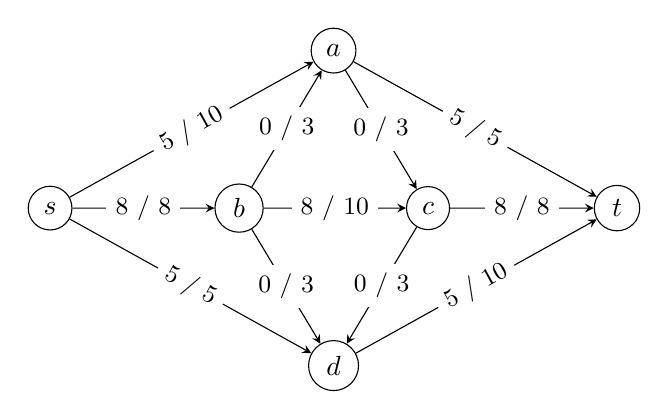
\begin{tikzpicture}[scale=0.8]
				\usetikzlibrary{arrows.meta}
				\node[draw,circle] (v0) at (4.5,  5)	    {$a$};
				\node[draw,circle] (v1) at (0,  2.5)    {$s$};
				\node[draw,circle] (v2) at (3,  2.5)	{$b$};
				\node[draw,circle] (v3) at (6,  2.5)    {$c$};
				\node[draw,circle] (v4) at (9,  2.5)	{$t$};
				\node[draw,circle] (v5) at (4.5,  0)    {$d$};
				
				\def\list {v1/v0/5/10, v1/v2/8/8, v2/v3/8/10, v3/v4/8/8, v0/v4/5/5}  % list elements
				\foreach \u\v\flow\weight in \list
				{	\draw[-stealth] (\u) -- (\v) node [fill=white, sloped, midway] {\small \flow\ $/$ \weight};
				}
				\def\vertical {v2/v0/0/3, v2/v5/0/3, v0/v3/0/3, v3/v5/0/3}  % list elements
				\foreach \u\v\flow\weight in \vertical
				{	\draw[-stealth] (\u) -- (\v) node [fill=white, midway] {\small \flow\ $/$ \weight};
				}
				\def\down {v1/v5/5/5, v5/v4/5/10} %list elements
				\foreach \u\v\flow\weight in \down
				{   \draw[-stealth] (\u) -- (\v) node [fill=white, sloped, midway] {\small \flow\ $/$ \weight};
				}
				
			\end{tikzpicture}
			\caption{\label{Fluss}}
		\end{center}
	\end{figure}
\end{aufgabe}

\begin{aufgabe}[Edmonds-Karp Algorithmus und capacity-scaling algorithm]
    % Algorithms and Data Structures 2 - networks2.pdf
    Benutze sowohl den Edmonds-Karp Algorithmus, als auch den \textit{capacity-scaling algorithm}, um in den folgenden beiden Graphen einen maximalen Fluss und einen minimalen Schnitt zu berechnen. Schreibe für jeden augmentierenden Pfad die Knoten auf dem Pfad und den Wert, um die der Pfad augmentiert wird, auf.
    
    \begin{figure}[ht]
    	\begin{minipage}[b]{0.5\textwidth}
    		\centering
    		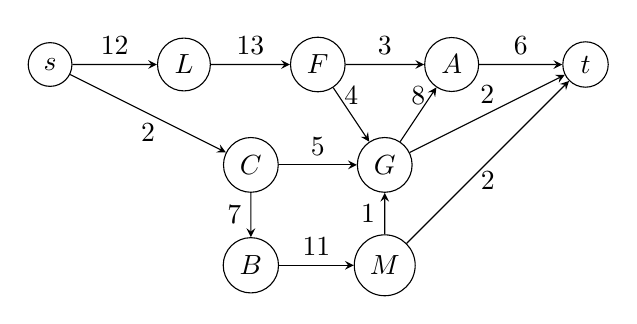
\begin{tikzpicture}[scale=0.85]
			\node[draw,circle] (v0) at (0,  3.5)	{$s$};
			\node[draw,circle] (v1) at (2,  3.5)    {$L$};
			\node[draw,circle] (v2) at (4,  3.5)	{$F$};
			\node[draw,circle] (v3) at (6,  3.5)    {$A$};
			\node[draw,circle] (v4) at (8,  3.5)	{$t$};
			\node[draw,circle] (v5) at (3,    2)    {$C$};
			\node[draw,circle] (v6) at (5,    2)    {$G$};
			\node[draw,circle] (v7) at (3,  0.5)    {$B$};
			\node[draw,circle] (v8) at (5,  0.5)    {$M$};
			
			\def\list {v0/v1/12, v1/v2/13, v2/v3/3, v3/v4/6, v2/v6/4, v5/v6/5, v6/v3/8,
			v6/v4/2, v7/v8/11}  % list elements
			\foreach \u\v\weight in \list
			{	\draw[-stealth] (\u) -- (\v) node [midway, above] {\weight};
			}
			\def\vertical {v5/v7/7, v8/v6/1 %v0/v4/3, v2/v5/4, v2/v9/4%, v3/v7/7, v6/v10/1, v11/v7/2
            }  % list elements
			\foreach \u\v\weight in \vertical
			{	\draw[-stealth] (\u) -- (\v) node [midway, left] {\weight};
			}
			\def\down {v0/v5/2, v8/v4/2} %list elements
			\foreach \u\v\weight in \down
			{   \draw[-stealth] (\u) -- (\v) node [midway, below] {\weight};
			}
		\end{tikzpicture}
    	\end{minipage}
    	\begin{minipage}[b]{0.5\textwidth}
    		\centering
    		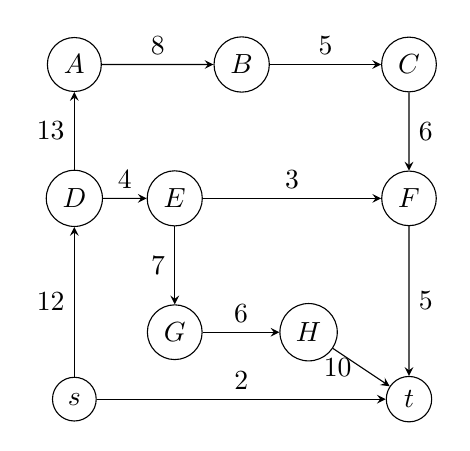
\begin{tikzpicture}[scale=0.85]
			\node[draw,circle] (v0) at (0  ,    0)	  {$s$};
			\node[draw,circle] (v1) at (0  ,    5)    {$A$};
			\node[draw,circle] (v2) at (2.5,    5)	  {$B$};
			\node[draw,circle] (v3) at (5  ,    5)    {$C$};
			\node[draw,circle] (v4) at (0  ,    3)	  {$D$};
			\node[draw,circle] (v5) at (1.5,    3)    {$E$};
			\node[draw,circle] (v6) at (5  ,    3)    {$F$};
			\node[draw,circle] (v7) at (1.5,    1)    {$G$};
			\node[draw,circle] (v8) at (3.5,    1)    {$H$};
			\node[draw,circle] (v9) at (5  ,    0)    {$t$};
			
			\def\list {v0/v4/12, v4/v1/13, v5/v7/7, v8/v9/10}  % label left from edge
			\foreach \u\v\weight in \list
			{	\draw[-stealth] (\u) -- (\v) node [midway, left] {\weight};
			}
			\def\vertical {v0/v9/2, v1/v2/8, v2/v3/5, v4/v5/4, v5/v6/3, v7/v8/6}  % label above edge
			\foreach \u\v\weight in \vertical
			{	\draw[-stealth] (\u) -- (\v) node [midway, above] {\weight};
			}
			\def\down {v3/v6/6, v6/v9/5} % label right from edge
			\foreach \u\v\weight in \down
			{   \draw[-stealth] (\u) -- (\v) node [midway, right] {\weight};
			}
		\end{tikzpicture}
    	
    	\end{minipage}
    \end{figure}
\end{aufgabe}

\begin{aufgabe}[Blutspende]
    % KT exercise 7.8
    Statistisch gesehen erhöht sich die Anzahl an Unfällen mit Beginn des Frühlings und damit auch der Bedarf an medizinischen Notfallbehandlungen, sodass auch vermehrt Bluttransfusionen notwendig sind. Stell dir vor, du arbeitest für ein Krankenhaus, das beurteilen muss, ob seine Blutreserven ausreichend sind.

    Beim Blutspenden gibt es eine grundlegende Regel: Eine Person hat in ihrem Blut bestimmte Antigene (du kannst dir Antigene als eine Art molekulare Signatur vorstellen). Bei einer Blutspende kann eine Person nur Blut empfangen, welches die gleichen Antigene hat, wie das eigene. Konkret gesagt unterteilt dieses Prinzip das Blut in vier Gruppen: A, B, AB und 0. Blutgruppe A hat das Antigen A, Blutgruppe B hat das Antigen B, Blutgruppe AB hat beide und Blutgruppe 0 hat keines der Antigene. Demnach können Patienten mit Blutgruppe A nur Blut der Gruppen A und 0, Patienten der Blutgruppe B nur Blut der Gruppen B und 0, Patienten der Blutgruppe 0 nur Blut der Gruppe 0 und Patienten der Blutgruppe AB Blut aller Blutgruppen empfangen.
    \begin{enumerate}
    	\item Seien $s_0,s_A,s_B$ und $s_{AB}$ die Vorräte des Krankenhauses an den vier Blutgruppen, angegeben in ganzen Einheiten. Nimm an, dass das Krankenhaus den prognostizierten Bedarf $d_0, d_A,d_B$ und $d_{AB}$ an Blut für die nächsten Wochen kennt. Gib einen Algorithmus an, der in Polynomialzeit auswertet, ob das vorrätige Blut den prognostizierten Bedarf der nächsten Woche deckt.
    	\item Schaue dir das folgende Beispiel an. Das Krankenhaus prognostiziert für die nächste Woche einen Bedarf von maximal $100$ Einheiten an Blut. Die durchschnittliche Verteilung der Blutgruppen über die U.S.-Bevölkerung liegt bei $45\%$ Blutgruppe 0, $42\%$ Blutgruppe A, $10\%$ Blutgruppe B und $3\%$ Blutgruppe AB. Das Krankenhaus möchte wissen, ob seine Vorräte ausreichend sind, wenn $100$ Patienten mit der erwarteten Verteilung über die Blutgruppen behandelt werden müssen. Es sind $105$ Einheiten an Blut vorrätig. Die Tabelle gibt den Vorrat und die Nachfrage an Blut an.
    	
    	\vspace{4mm}
    	\begin{center}
    	\begin{tabular}{|c|c|c|}
    	\hline 
    	Blutgruppe & Vorrat & Nachfrage \\ 
    	\hline 
    	0 & 50 & 45 \\ 
    	\hline 
    	A & 36 & 42 \\ 
    	\hline 
    	B & 11 & 10 \\ 
    	\hline 
    	AB & 8 & 3 \\ 
    	\hline 
    	\end{tabular}
    	\end{center}
    	\vspace{4mm}
    	Sind die 105 vorrätigen Einheiten an Blut ausreichend, um der Nachfrage von $100$ Einheiten gerecht zu werden? Finde eine Verteilung, sodass die maximale Anzahl an Patienten behandelt werden kann. Benutze einen minimalen Kapazitäten-Schnitt, um zu begründen, warum nicht alle Patienten behandelt werden können. Stelle außerdem eine verständliche Erklärung dieses Umstandes für die Mitglieder der Krankenhausverwaltung bereit, die ALGO2 nicht belegt haben. (Beispielsweise soll deine Erklärung die Worte \textit{Fluss, Schnitt} oder \textit{Graph} nicht in dem Sinne enthalten, wie wir sie in der Vorlesung benutzen.)
    \end{enumerate}
    \vspace{4mm}
    Möchtest auch du helfen, die Vorräte des Krankenhauses aufzufüllen? Dann informiere dich hier: \url{https://www.blutspende.de}
\end{aufgabe}

\begin{aufgabe}[Weihnachtsbäume]
    % Algorithms and Data Structures 2 - networks2.pdf
    Professor Regloh hat dich beauftragt, die jährliche Weihnachtsfeier für alle Student:innen der Goethe-Universität zu organisieren. Du musst einen Plan erstellen, auf dem die Platzierung der Tische im Casino-Festsaal vermerkt ist. Damit die Brandschutzmaßnahmen eingehalten werden können, hat die Frankfurter Feuerwehr den Festsaal in ein quadratisches $n \times m$ Gitter aufgeteilt und festgelegt, dass höchstens zwei Tische in jeder Zeile und höchstens ein Tisch in jeder Spalte aufgestellt werden dürfen. Leider liebt Professor Regloh Weihnachtsbäume so sehr, dass er in vielen Bereichen schon welche aufgestellt hat. Du kannst keinen Tisch in einen Bereich stellen, in dem schon ein Weihnachtsbaum steht.
    
    \textbf{Beispiel.} Es gilt $n = 4$ und $m = 8$. Die $\star$ stellen Weihnachtsbäume dar und $T$ die Tische. In diesem Beispiel ist die maximale Anzahl an platzierbaren Tischen 7.
    
    \vspace{4mm}
    \begin{center}
    \begin{tabular}{|c|c|c|c|c|c|c|c|}
    \hline 
    \rule[-1ex]{0pt}{2.5ex} $\star$ & $T$ &  &  &  &  &  & $T$ \\ 
    \hline 
    \rule[-1ex]{0pt}{2.5ex} $T$ & $\star$ & $\star$ & $T$ & $\star$ & $\star$ &  & $\star$ \\ 
    \hline 
    \rule[-1ex]{0pt}{2.5ex}  & $\star$ & $\star$ &  & $\star$ & $\star$ & $T$ & $\star$ \\ 
    \hline 
    \rule[-1ex]{0pt}{2.5ex}  & $\star$ & $T$ & $\star$ &  & $T$ & $\star$ &  \\ 
    \hline 
    \end{tabular} 
    \end{center}
    \vspace{4mm}
    \begin{enumerate}
    	\item Modelliere das Problem als Graphenproblem. Erkläre, wie du das machst und zeichne den zum oben angegebenen Beispiel passenden Graphen.\\
    	\item Beschreibe einen Algorithmus, der, gegeben $n,m$ und die Platzierung der Weihnachtsbäume, eine maximale Anzahl an Tischen, die im Festsaal platziert werden können, ausgibt. Analysiere die asymptotische Laufzeit deines Algorithmus. Denke daran, die Korrektheit deines Algorithmus zu zeigen.\\
    	\item Implementiere deinen Algorithmus in Python oder Java.
    \end{enumerate}
\end{aufgabe}

\section*{Donnerstag}

\begin{aufgabe}[Fluchtwege]
    % KT exercise 7.14
    Wir definieren das Fluchtproblem wie folgt: Gegeben ist ein gerichteter Graph $G = (V,E)$ (stell dir ein Straßennetzwerk vor). Eine Teilmenge $X \subset V$ aller Knoten sind bewohnte Knoten und eine andere Teilmenge $S \subset V$ sind sichere Knoten. Du kannst annehmen, dass $X$ und $S$ disjunkt sind. Für den Notfall soll es Fluchtwege von den bewohnten Knoten zu den sicheren Knoten geben. Eine Menge von Fluchtwege ist als eine Menge von Pfaden in $G$ definiert, sodass $1.$ jeder Knoten aus $X$ der Anfang eines Pfades ist, $2.$ der letzte Knoten eines Pfades in $S$ liegt und $3.$ die Pfade keine gemeinsamen Kanten besitzen. Diese Menge an Pfaden sorgt dafür, dass die bewohnten Knoten sicher evakuiert werden können, ohne dass eine Kante in $G$ überlastet wird.
    \begin{enumerate}
    	\item Gegeben $G, X$ und $S$. Zeige, wie man in polynomialer Zeit entscheiden kann, ob eine solche Menge an Fluchtwege existiert.
    	\item Wir wollen das gleiche Problem lösen, wie in a), aber mit einer strengeren Version der $3.$ Bedingung. Die Pfade dürfen nun auch keine gemeinsamen Knoten mehr haben.
    	
    	Zeige, ob mit dieser neuen Bedingung in polynomialer Zeit entschieden werden kann, ob eine Menge an Fluchtwege existiert.
    	
    	Gib außerdem ein Beispiel mit gleichem $G, X$ und $S$ an, das in Aufgabenteil a) \glqq Ja\grqq{} ausgibt und in Aufgabenteil b) \glqq Nein\grqq.
    \end{enumerate}
\end{aufgabe}

\begin{aufgabe}[Eulerkreise in gemischten Graphen]
    % Algorithms and Data Structures 2 - networks2.pdf
    Es ist bekannt, dass ein stark zusammenhängender Graph einen Eulerkreis (ein Kreis, der jede Kante genau einmal enthält) besitzt genau dann, wenn jeder Knoten die gleiche Anzahl eingehender und ausgehender Kanten hat.
    
    Im Folgenden arbeiten wir mit gemischten Graphen. Das sind Graphen, in denen einige Kanten gerichtet sind und einige ungerichtet. Wir nehmen an, dass die Graphen zusammenhängend sind. Beispielsweise sind die Graphen zusammenhängend, wenn die Richtung aller Kanten ignoriert wird.
    
    Wir wollen einen Algorithmus haben, der entscheidet, ob es möglich ist, den ungerichteten Kanten eine Richtung zu geben, sodass der Graph einen Eulerkreis besitzt. Im Beispiel können die ungerichteten Kanten des gemischten Graphen links so gerichtet werden, dass ein Eulerkreis entsteht (die Nummern der Kanten geben die Besuchsreihenfolge an).
    
    \begin{figure}[ht]
    	\begin{minipage}[b]{0.5\textwidth}
    		\centering
    		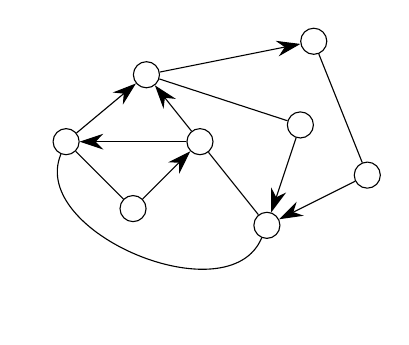
\begin{tikzpicture}[scale=0.85]
			\node[draw,circle] (v0) at (0,  0)  {};
			\node[draw,circle] (v1) at (1,  -1)  {};
			\node[draw,circle] (v2) at (1.2, 1)  {};
			\node[draw,circle] (v3) at (2,  0)  {};
			\node[draw,circle] (v4) at (3,  -1.25)  {};
			\node[draw,circle] (v5) at (3.5, 0.25)  {};
			\node[draw,circle] (v6) at (3.7,  1.5)  {};
			\node[draw,circle] (v7) at (4.5,  -0.5)  {};
			
			\def\list {v0/v2, v1/v3, v2/v6, v3/v0, v3/v2, v5/v4, v7/v4}  % directed edges
			\foreach \u\v in \list
			{	\draw[-{Stealth[length=3mm, width=2mm]}] (\u) -- (\v);}
			
			\def\vertical {v0/v1, v2/v5, v3/v4, v6/v7}  % undirected edges
			\foreach \u\v in \vertical
			{	\draw[] (\u) -- (\v);}
			
			\path (v0) edge[bend right=90] node [left] {} (v4);
		\end{tikzpicture}
    	\end{minipage}
    	\begin{minipage}[b]{0.5\textwidth}
    		\centering
    		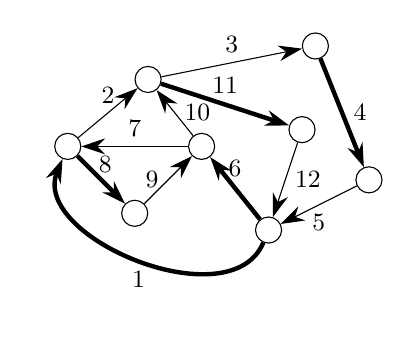
\begin{tikzpicture}[scale=0.85]
			\node[draw,circle] (v0) at (0,  0)  {};
			\node[draw,circle] (v1) at (1,  -1)  {};
			\node[draw,circle] (v2) at (1.2, 1)  {};
			\node[draw,circle] (v3) at (2,  0)  {};
			\node[draw,circle] (v4) at (3,  -1.25)  {};
			\node[draw,circle] (v5) at (3.5, 0.25)  {};
			\node[draw,circle] (v6) at (3.7,  1.5)  {};
			\node[draw,circle] (v7) at (4.5,  -0.5)  {};
			
			\path (v4) edge[-{Stealth[length=3mm, width=2mm]}, ultra thick, bend left=90] node [font=\small,midway, below] {$1$} (v0);
			\path (v0) edge[-{Stealth[length=3mm, width=2mm]}							] node [font=\small,midway, above] {$2$} (v2);
			\path (v2) edge[-{Stealth[length=3mm, width=2mm]}							] node [font=\small,midway, above] {$3$} (v6);
			\path (v6) edge[-{Stealth[length=3mm, width=2mm]}, ultra thick				] node [font=\small,midway, right] {$4$} (v7);
			\path (v7) edge[-{Stealth[length=3mm, width=2mm]}							] node [font=\small,midway, below] {$5$} (v4);
			\path (v4) edge[-{Stealth[length=3mm, width=2mm]}, ultra thick				] node [font=\small,midway, above] {$6$} (v3);
			\path (v3) edge[-{Stealth[length=3mm, width=2mm]}							] node [font=\small,midway, above] {$7$} (v0);
			\path (v0) edge[-{Stealth[length=3mm, width=2mm]}, ultra thick				] node [font=\small,midway, above,yshift=-1.5, xshift=1.5] {$8$} (v1);
			\path (v1) edge[-{Stealth[length=3mm, width=2mm]}							] node [font=\small,midway, left ] {$9$} (v3);
			\path (v3) edge[-{Stealth[length=3mm, width=2mm]}							] node [font=\small,midway, right] {$10$} (v2);
			\path (v2) edge[-{Stealth[length=3mm, width=2mm]}, ultra thick				] node [font=\small,midway, above] {$11$} (v5);
			\path (v5) edge[-{Stealth[length=3mm, width=2mm]}							] node [font=\small,midway, right] {$12$} (v4);
			
		\end{tikzpicture}
    	
    	\end{minipage}
    \end{figure}
    
    Gib einen Algorithmus an, der entscheidet, ob man alle ungerichteten Kanten so richten kann, dass ein Eulerkreis entsteht.
    
    \textit{Hinweis:} Denk an einen bipartiten Graphen, bei dem auf der einen Seite die Knoten aus $G$ und auf der anderen Seite die Kanten aus $G$ dargestellt sind. Nutze den Algorithmus der vorherigen Aufgabe.
\end{aufgabe}

\begin{aufgabe}[Puzzle der Woche: Das Zwölf-Münzen Problem]
	% Algorithms and Data Structures 2 - networks2.pdf
	Vor dir liegen 12 Münzen. 11 davon sind identisch, aber eine ist schwerer oder leichter als der Rest. Du hast eine traditionelle Balkenwaage mit zwei Waagschalen. Um die Waage zu benutzen, legst du eine Münze in jede Schale. Die Waage zeigt dann an, welche der beiden Seiten (und damit welche der beiden Münzen) schwerer ist. Die Balkenwaage darf dreimal benutzt werden, um die andere Münze zu finden und um festzustellen, ob diese leichter oder schwerer ist als der Rest.
\end{aufgabe}

\end{document}
